%%%%%%%%%%%%%%%%%%%%%%%%%%%%%%%%%%%%%%%%%%%%%%
\section{TPC Charge Extraction}
\label{sec:tpc-signal-calibration}

In Section~\ref{sec:tpc_signal_formation}, the signal formation in TPC
is described. This section describes the procedure of the TPC 
charge extraction. As shown in Figure~\ref{fig:signal_formation}, the 
goal of TPC charge extraction is to recover the number of ionized 
electrons from the digitized TPC signal. 

%%%%%%%%%%%%%%%%%%%%%%%%
\subsection{Deconvolution Technique}\label{sec:decon}
\label{sec:decon-tech}
Deconvolution is a mathematical technique to extract a \textit{real signal}
$S(t)$ from a \textit{measured signal} $M(t_0)$. The deconvolution technique 
was introduced to LArTPC signal processing in LarSoft by Bruce Baller in the 
context ArgoNEUT data analysis~\cite{bruce}. 
\fixme{include names in content?}
The goal of the deconvolution is 
to ``remove'' the field and electronics response functions from the measured 
signal to recover the number of ionized electrons.~\footnote{Strictly speaking,
the deconvolution replaces the bipolar response function with a unipolar smearing
function.} This technique has the advantages of being robust and fast and is an 
essential step in the overall charge extraction process. 

The measured signal is modeled as a convolution integral over the real 
signal $S(t)$ and a given detector \textit{response function} $R(t,t_0)$ which gives the
instantaneous portion of the measured signal at some time $t_0$ due to
an element of real signal at time $t$.
\begin{equation}\label{eq:decon_1}
M(t_0) = \int_{-\infty}^{\infty}  R(t,t_0) \cdot S(t) \cdot dt.
\end{equation}
If the detector response function only depends on the relative time 
difference between $t$ and $t_0$, the above equation can be solved by 
doing a Fourier transformation on both sides of the equation:
\begin{equation}
M(\omega) = R(\omega) \cdot S(\omega), 
\end{equation}
where $\omega$ is the frequency. In this case, we can derive the signal in the 
frequency domain by taking the ratio of measured signal and the given
response function:
\begin{equation}\label{eq:decon_2}
S(\omega) = \frac{M(\omega)}{R(\omega)}.
\end{equation}
The real signal in the time domain can then be obtained by applying the 
inverse Fourier transformation from the frequency domain. 

The Shockley-Ramo response function $R(\omega)$ does not address
contributions to the measured signal which are due to real world
sources of electrical \textit{noise} from thermal and unwanted transmitting
sources or due to the approximation in the digitization.
Such contributions to $M(\omega)$ will not be ``divided out'' by the deconvolution.
Worse, because the response function becomes small (see Section~\ref{sec:decon-2D-ind}) %below) 
at low 
frequencies for the induction planes and at high frequencies for all
planes, the noise components in these frequencies will become
enhanced by the deconvolution.

To address the problem of noise, a \textit{filter function} $F(\omega)$ is
introduced.  Its purpose is to attenuate the problematic noise.  The
addition of this function can be considered an augmentation to the
response function, which may in any case be chosen freely as it is a model.  
The two functions are kept distinct for clarity in the notation here.
Equation~\ref{eq:decon_2} is then updated to become
\begin{equation}\label{eq:decon_filt}
S(\omega) = \frac{M(\omega)}{R(\omega)} \cdot F(\omega).
\end{equation}
With a suitable noise model, an improved estimator for the signal
$S(t)$ in the time domain can then be found by applying an inverse Fourier 
transform to $S(\omega)$.  Essentially, the deconvolution replaces the field and 
electronics response function with the filter response function. The 
advantage of this procedure shows up on the induction plane where the irregular bipolar 
field response function is replaced by a regular unipolar response function through
the inclusion of the software filter. 


%%%%%%%%%%%%%%%%%%%%%%%%
\subsection{Importance of 2D Deconvolution for Induction Planes}
\label{sec:decon-2D-ind}

The 1D deconvolution procedure described in Section~\ref{sec:decon-tech} %the previous section 
works well in dealing with signal in the collection wire plane, but is not 
optimal when applied to signals in the induction wire planes. 
As described in Section~\ref{sec:tpc_signal_formation}, the induction plane wire 
signal receives contributions not only from ionization charge 
passing by the wire of interest, but also from ionization charge drifting in 
nearby wire boundaries. In addition, within the boundary of the wire of 
interest, the value of the field response function varies appreciably 
 so at small scales the location of the drifting charge relative to the wire 
is important. In this case, Equation~\ref{eq:decon_1} would naturally expand to 
\begin{equation}\label{eq:decon_2d_1}
M_i(t_0) = \int_{-\infty}^{\infty} \left( R_0 \cdot (t-t_0) \cdot S_i(t) + 
R_1 \cdot (t-t_0) \cdot S_{i+1} (t) + ...\right) \cdot dt,
\end{equation}
where $M_i$ represents the measured signal from wire $i$.  $S_i$ and
$S_{i+1}$ represents the real signal in the boundaries of wire $i$ and
its next neighbor, respectively.
The $R_0$ represents the average response function for an ionization
charge passing through the wire boundary of interest.
Similarly, the $R_1$ represents the average response function for an
ionization charge drifting past in the next adjacent wire boundary. One can
easily expand this definition to some number of neighbors by introducing terms up 
to $R_{n-1}$.

If we then apply a Fourier transformation on both sides of Equation~\ref{eq:decon_2d_1},
we have:
\begin{equation}\label{eq:decon_2d_2}
M_i(\omega) = R_0(\omega) \cdot S_i(\omega) + R_1(\omega) \cdot S_{i+1} (\omega) + ...,
\end{equation} 
which can be written in a matrix notation as:
\begin{equation}
\begin{pmatrix}
    M_1(\omega)\\
    M_2(\omega)\\
    \vdots\\
    M_{n-1}(\omega)\\
    M_{n}(\omega)
\end{pmatrix}
=
\begin{pmatrix}
R_0(\omega) & R_1(\omega) & \ldots & R_{n-2}(\omega) & R_{n-1}(\omega) \\
R_1(\omega) & R_0(\omega) & \ldots & R_{n-3}(\omega) & R_{n-2}(\omega) \\
    \vdots  & \vdots      & \ddots & \vdots          & \vdots \\
    R_{n-2}(\omega) & R_{n-3}(\omega) & \ldots & R_0(\omega) & R_1(\omega) \\
    R_{n-1}(\omega) & R_{n-2}(\omega) & \ldots & R_1(\omega) & R_0(\omega) \\
\end{pmatrix}
\cdot
\begin{pmatrix}
    S_1(\omega)\\
    S_2(\omega)\\
    \vdots\\
    S_{n-1}(\omega)\\
    S_{n}(\omega)
\end{pmatrix}
\label{eq:matrix_expansion}
\end{equation}
Now, if we assume that we know response functions (i.e., the matrix $R$), the 
problem converts into deducing the vector of $S$ with the measured signal $M$. 
%
This can be achieved by inverting the matrix $R$. In practice and away
from plane edges the matrix $R$ is taken to be symmetric and its
inversion can again be achieved by the FFT.
%
As this expands the 1D deconvolution (with respect to the time axis)
into a 2D deconvolution (with respect to both the time and wire
axes), similarly we must also expand the filter function to cover
both time and wire dimensions.

A comment on the limitation (or approximation) 
assumed in the 2D deconvolution is needed. As shown in Equation~\ref{eq:decon_2d_1}, the 
average response functions are used in describing the measured signal. These 
ignore the detailed position dependence of the response function. 
This approximation ignores the fine-grained but clear position
dependence in the calculated weighting fields.
However, since we can only measured the signal from any given wire as
a function of time, there is no additional information to be used to
resolve the ionization electron distributions within a wire boundary.
This technique can in principle be improved to include the position-dependent
response once the local ionization charge distribution is roughly reconstructed. 

%%%%%%%%%%%%%%%%%%%%%%%%
\subsection{Additional Challenges in Deconvolution}

\begin{cdrfigure}[Simulated field response functions in the time and frequency domains]{induction_field}{(left) Simulated field response functions for induction (black and red) and 
collection (blue) wires are shown in the time domain. (right) The same are shown in 
the frequency domain.}
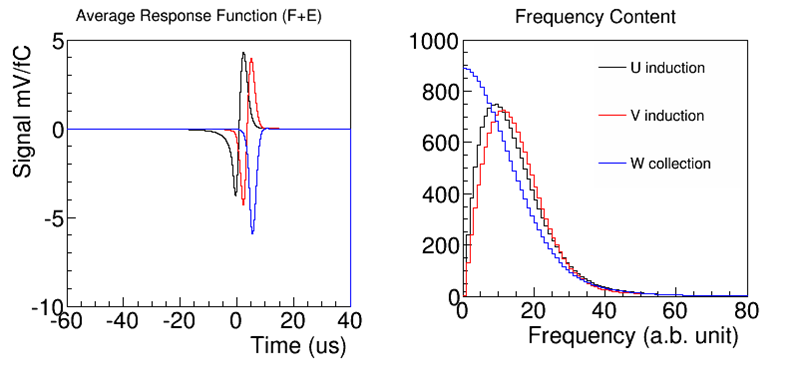
\includegraphics[width=0.95\textwidth]{induction_field_response.png}
\end{cdrfigure}


The 1D and 2D deconvolution procedures provide a robust method to extract the ionization
electrons for the collection and induction planes, respectively. 
%
While working well for the collection plane, the procedure is still not optimal 
for the induction plane due to the nature of the induction plane signal. 
Figure~\ref{fig:induction_field} shows the field response as simulated by Garfield \fixme{citation?}
for induction and collection wire planes and point ionization
electrons. While the field response for the collection wire plane is unipolar, the field 
response for the induction wire plane is bipolar. 
%
The early, negative half corresponds to the ionization electron moving
towards the wire plane and the late, positive half corresponds
to the ionization electron moving away.
%
The integration of the field response function is close to zero
as the bias wire voltages are applied such that that none of the ionization electrons are
collected. The right panel of Figure~\ref{fig:induction_field} shows the 
frequency components of the field response. 
%
Since an induction plane field response has a bipolar shape in the time domain 
there is a corresponding suppression at low frequency in the frequency 
domain. At zero frequency, the frequency component essentially gives the 
integration of field response function over time and thus should be near 
zero (again, because no charge is collected).


The suppression of the induction field response at low frequency is problematic for the
proposed deconvolution procedure. First,  the measured signal contains the electronic noise, 
which usually increases at low frequency (the so-called 1/f noise). Therefore, as shown in 
Equation~\eqref{eq:decon_filt}, the low-frequency noise will be amplified in the deconvolution 
process, since the denominator (i.e., the induction field response) is generally small at 
low frequency. This can be seen clearly in Figure~\ref{fig:decon_example}, where the low-frequency noise
is significant. The large low-frequency noise would lead to large uncertainty 
in the charge estimation, and needs to be dealt with.  

\begin{cdrfigure}[Example of deconvoluted spectrum for the induction plane (simulation)]{decon_example}{Example of deconvoluted spectrum for the induction plane (simulation).}
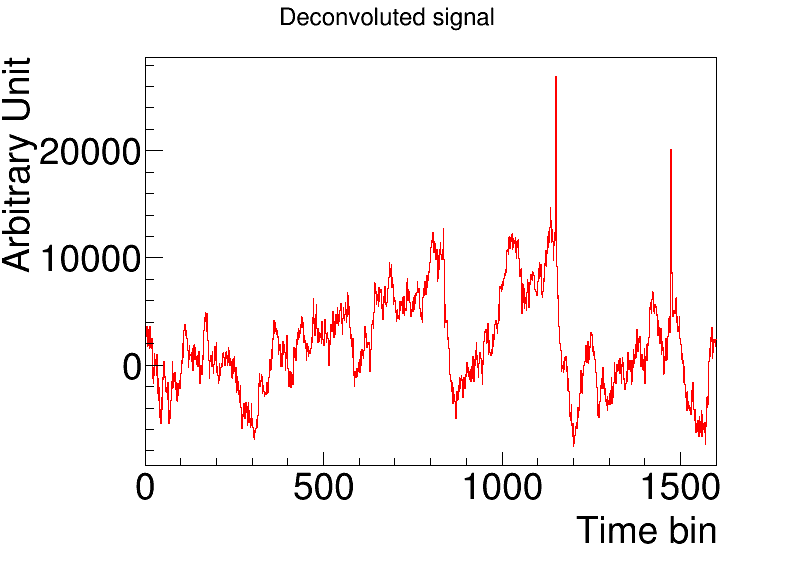
\includegraphics[width=0.8\textwidth]{decon_example.png}
\end{cdrfigure}


In Equation~\eqref{eq:decon_filt}, a frequency-domain  filter function is introduced 
to suppress the numerical instability caused by the presence of noise. One can imagine using % to use 
this
software filter to suppress the electronic noise at low frequency. This is also 
not acceptable due to large distortion introduced on the signal. \fixme{previous sentence unclear (``also not acceptable'' relative to what?)} To understand this 
point, we recall that the software filter is effectively a smearing function. 
Figure~\ref{fig:low_f_filter} shows an illustrative real signal (left), its convolution 
with a low-frequency filter (middle), and the low-frequency filter itself (right). 
It is obvious that the signal is strongly distorted due to the application of the 
low-frequency software filter. 

\begin{cdrfigure}[Impact of the low-frequency filter]{low_f_filter}{The impact of the low-frequency filter (right). The unit of the $x$-axis 
is MHz.  The real signal and the convoluted signal are shown in the left and
middle panels, respectively. A time tick is 0.5 $\mu s$.}
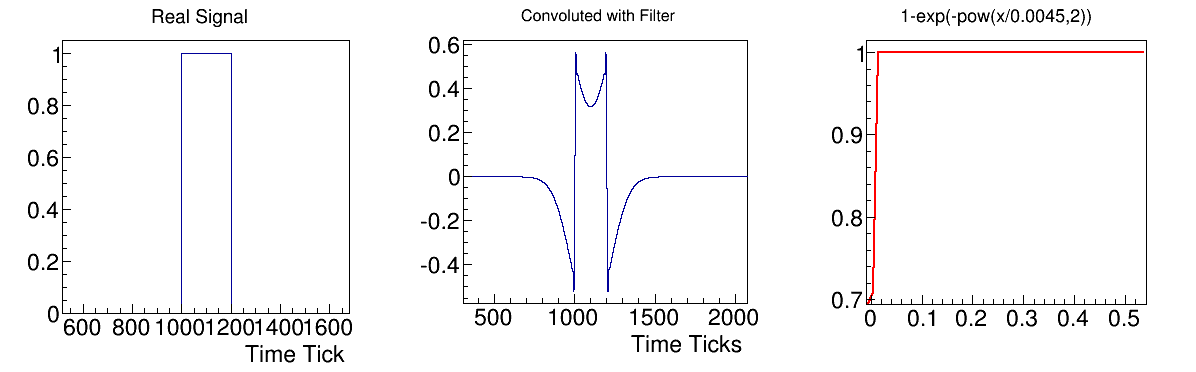
\includegraphics[width=0.95\textwidth]{low_freq.png}
\end{cdrfigure}

In order to deal with this problem, we turn to using two techniques in the time domain: 
\textit{region of interest (ROI)} and \textit{adaptive baseline (AB)}. The ROI technique
was proposed by Bruce Baller \fixme{name again} in the context of reducing data size and speeding up the 
deconvolution process. At the same time, the ROI technique can %also 
be used to 
suppress the low-frequency noise. In order to recognize this point, we consider
a time window with $N$ time ticks.  For ProtoDUNE-SP, this would be a window of 
$N\times0.5\mu\mbox{s}$. The highest frequency that can be resolved with such 
sampling would be 1~MHz. The first discrete frequency above zero would be $2/N$ MHz, 
and no result within the ROI can be sensitive to any noise components below this 
frequency.  Therefore, if we can identify the signal region and create a ROI to 
cover the signal, we can naturally suppress the low-frequency noises. 

The adaptive baseline (AB) technique was introduced by Mike Mooney  \fixme{name again} 
in the context of 
dealing with the ASIC saturation observed in MicroBooNE. The AB is essentially a 
local baseline calculated in a given a ROI. However, instead of a simple average of 
the baseline at the start and end points of a ROI, a linear interpolation is used to 
correct the baseline. Given the two constraints (start and end points of the ROI), 
the linear interpolation with two degrees of freedom is the best that one can achieve 
to remove bias in the baseline. 

In Section~\ref{sec:decon-frf-calc} %the following, 
we describe various parts \fixme{better word than `parts'? maybe `techniques'?} used in the charge extraction.

%%%%%%%%%%%%%%%%%%%%%%%%
\subsection{Calculation of Field Response Function}
\label{sec:decon-frf-calc}

The field response is calculated by Garfield~\cite{garfield} \fixme{name again}  in a 22-cm (along the 
field direction) $\times$ 30-cm (along the wire plane direction) region in 2D.  
In the drift direction, the grid plane is labeled as G, the two induction %planes 
wire 
planes are labeled U and V, and the collection plane is W.  The spacing between the wire 
planes is 4.76~mm. The bias voltages of-665 V, -370 V, 0 V, and +820 V for the G, U, V, and 
W planes, respectively, are configured according the operating conditions that ensure 100\%
    transmission of ionization electrons through the first two induction planes.  
    101 wires of diameter 150 $\mu$m are set on each wire plane with a pitch of 4.667 (4.79 for collection) mm.  A ground plane is placed 1~cm behind the W plane.  The drift
    field is uniform with 500~V/cm. The electron drift velocity as a function of
    electric field is taken from measurements~\cite{Li:2015rqa,lar_property}
    instead of using the default velocity table contained in~\cite{garfield}. % Garfield. 
    The electron
    diffusion is turned off in the simulation. The field response function then can
    be calculated for each individual wire in the form of induction current 
    (U and V planes) and collection current on (W planes) as a function of time for
    an electron drift which starts from arbitrary position within the region of calculation. 
    \fixme{please clarify previous sentence. Here is my attempt to make it less of a mouthful:
    
 For an electron drift that starts from an arbitrary position within the ROI, the field response then can
    be calculated for each individual wire in the form of induction current 
    (U and V planes) or collection current (W plane) as a function of time.
    }
    
    
    Figure~\ref{fig:garfield_2d} shows the configuration used in Garfield 2D simulation.
The Garfield-simulated response functions are shown in Figure~\ref{figs:overall_response}.
 The average response function for single electrons within a wire region 
is calculated for the closest wire $R_0$, next adjacent wire $R_1$, and so on. The U and 
V plane response functions are shown in the middle and right panel of 
Figure~\ref{figs:overall_response}, respectively.  For induction wire planes, these response 
functions are reasonably balanced, as expected.


\begin{cdrfigure}[Description of the Garfield 2D simulation of field response 
functions]{garfield_2d}{Description of the Garfield 2D simulation of field response functions}
  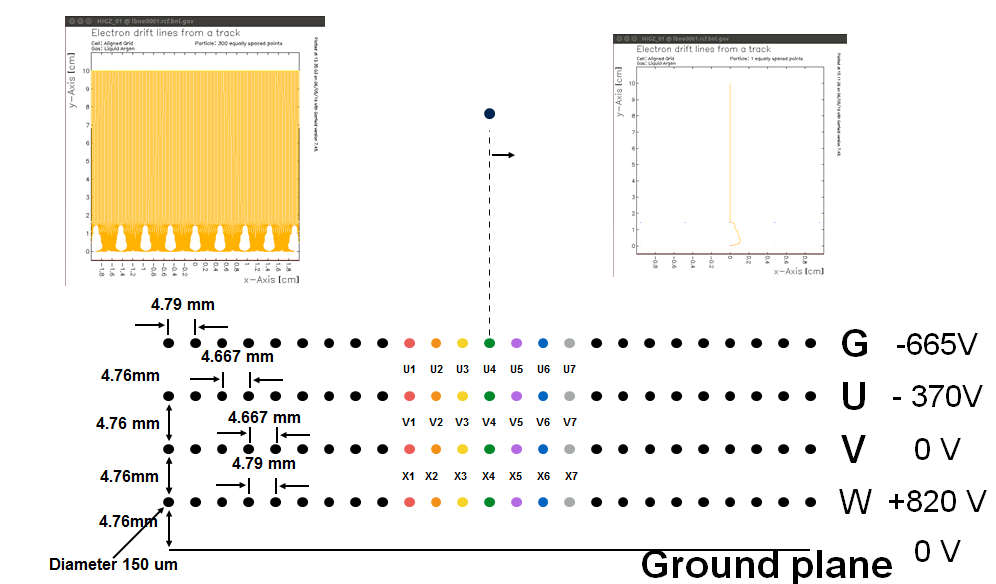
\includegraphics[width=0.95\textwidth]{Garfield_simu.png}
\end{cdrfigure}
\fixme{Figure~\ref{fig:garfield_2d} needs a more descriptive caption}


\begin{cdrfigure}[Overall response functions]{overall_response}{The overall response functions, i.e., %which is 
the convolution of the
electronics response function (14 mV/fC gain and 2 $\mu$s shaping time) 
and the field response.}
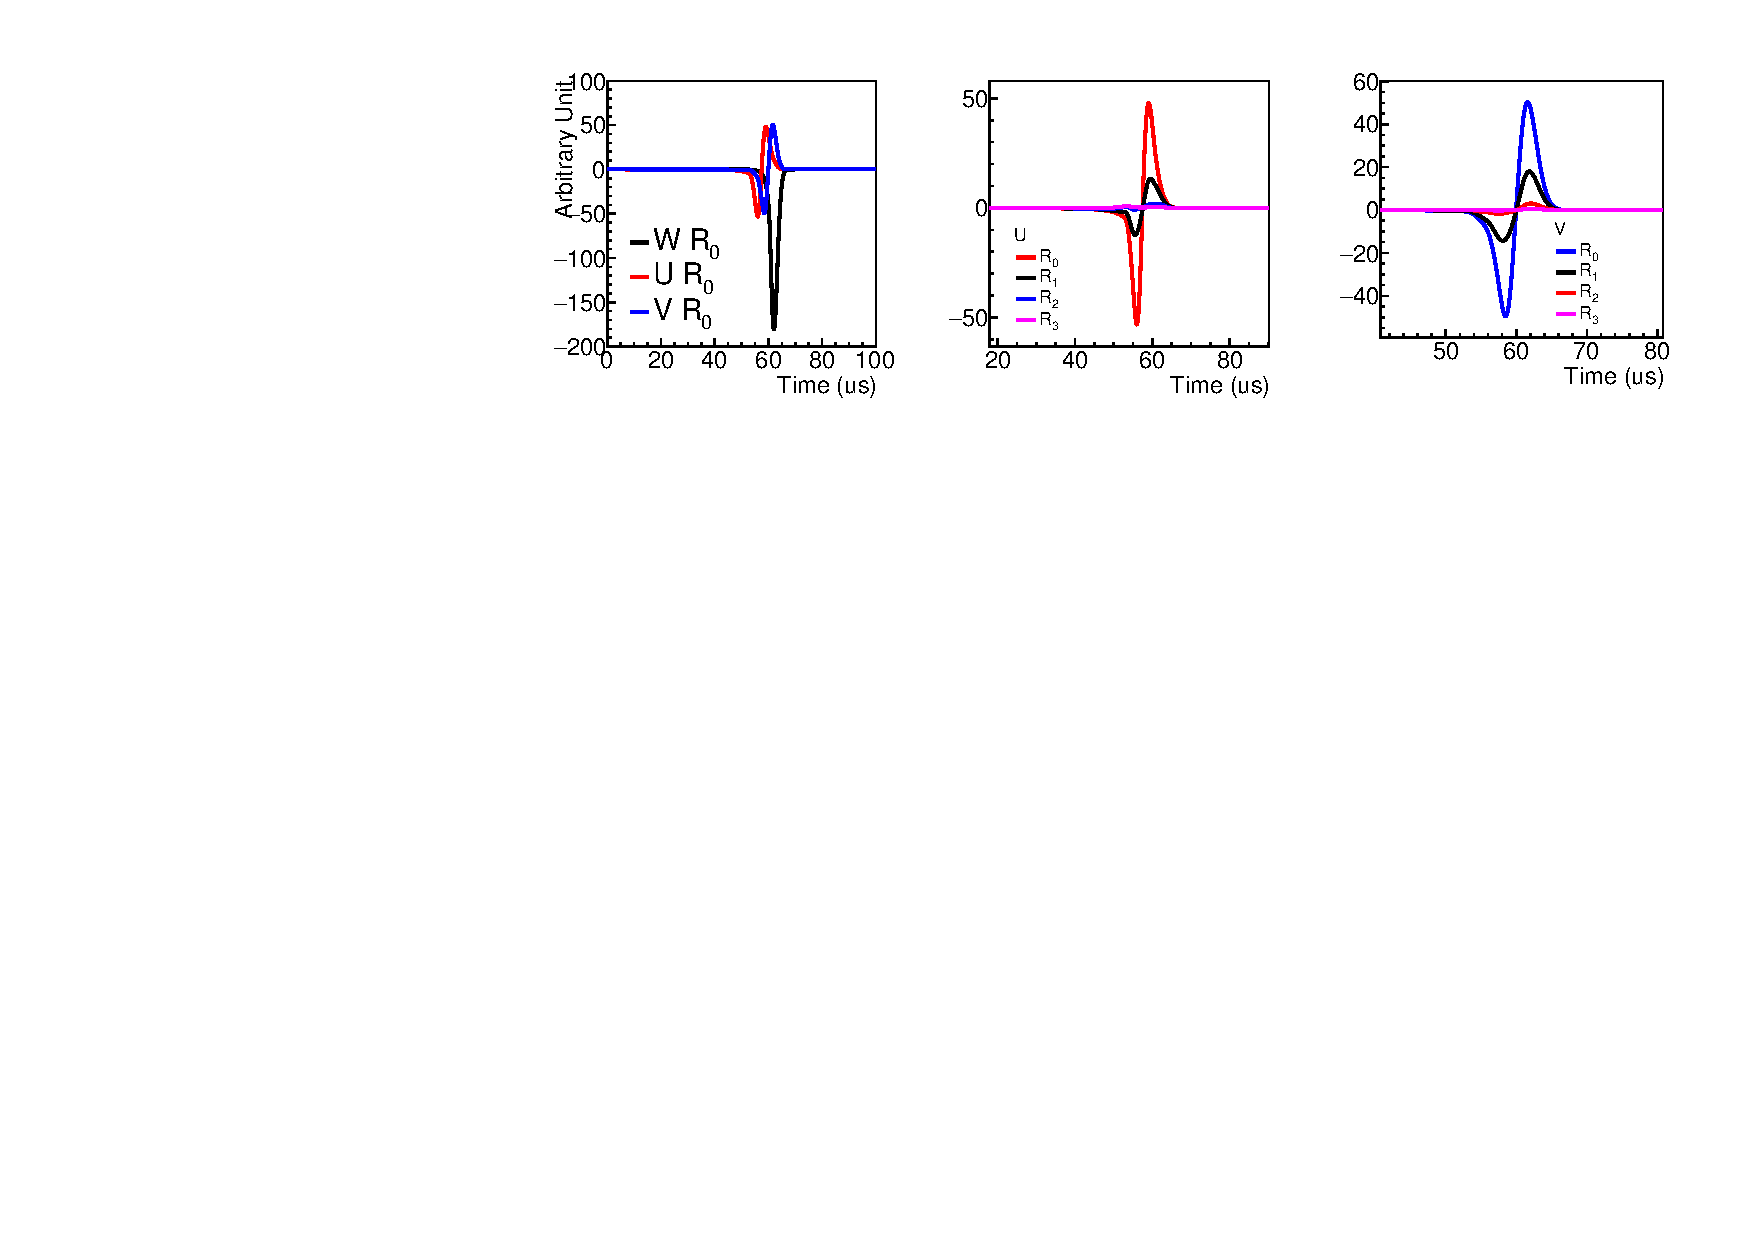
\includegraphics[width=0.95\textwidth]{dune_field_res.pdf}
\end{cdrfigure}
\fixme{This could use more description, but I guess it's clear what each panel is}

%%%%%%%%%%%%%%%%%%%%%%%%
\subsection{Choice of Software Filter}

Two types of filters are selected and implemented.  The first, inspired by the Wiener filter,  
 is modified to not suppress low-frequency components.  The second is the 
Gaussian filter. While the first one is optimized \fixme{independently?} for each wire plane to produce a 
high signal-to-noise ratio, the second one is optimized for the three planes as a group % and same to all the planes 
to correctly estimate the charge which is independently measured on each  plane. %of the three planes.  
This latter is important if all three planes are used for energy measurement 
and is critical for proper application of the Wire-Cell imaging technique~\cite{wire-cell}.  
In this section, we describe the selection process that resulted in %choice on 
these software filters.

The standard Wiener noise filter~\cite{wiener} is constructed using the expected 
signal $S(\omega)$ and noise $N(\omega)$ frequency spectra:
\begin{equation}
F(\omega) = \frac{S^2(\omega)}{S^2(\omega) + N^2(\omega)}.
\end{equation}
With this construction, the Wiener filter is expected to achieve the best signal-to-noise ratio. 
However, applying the Wiener filter to TPC signal processing is problematic. 
First, in a LArTPC, the TPC signal $S(\omega)$ varies substantially
depending on the exact nature of the event topology.
Second, the electronic noise spectrum is a function of the time window
over which it is observed. A longer time window allows for observation
of more low-frequency noise components.
Third, the induction wire signal spectrum is small at low frequency
and so would be its \fixme{own?} Wiener filter.  However, as discussed previously, 
a software filter with low-frequency suppression leads to large distortions 
of the signal and is thus not ideal.  

The functional form of the software filter is chosen as:
\begin{equation}
F(\omega) = 
\begin{cases}
e^{- \frac{1}{2} \cdot \left( \frac{\omega}{a} \right)^b} &  \omega >0 \\
0 &  \omega = 0, \\
\end{cases}
\end{equation}
where $a$ and $b$ are two free parameters.  Note, $b=2$ is basically the Gaussian filter. 
The filter is explicitly zero at $\omega = 0$ in order to remove the DC component in the 
deconvoluted signal. This removes information about the baseline;  a new baseline is 
calculated and restored for the waveform after deconvolution. The above functional form 
of the filter has another advantageous property:
\begin{equation}
lim_{\omega \rightarrow 0} F(\omega) = 1.
\end{equation}
which means the integral of the smearing function is unity, which does not introduce any
extra factor in the overall normalization. The free parameters $a$ and $b$ in the above 
form are determined by matching the tail of Wiener filter at its high-frequency side. 
An example of a software filter is shown in Figure~\ref{fig:soft_filter_1}. 

\begin{cdrfigure}[Wiener-inspired filter and Gaussian filter used in the 2D deconvolution]{soft_filter_1}{The Wiener-inspired filter and Gaussian filter used in the 2D deconvolution. 
The time and frequency domain content are shown on the left and right panel, respectively.
The x-axis's unit for the time domain is $\mu$s. For the frequency domain, the number 2000
corresponds to $\sim$0.42 MHz.}
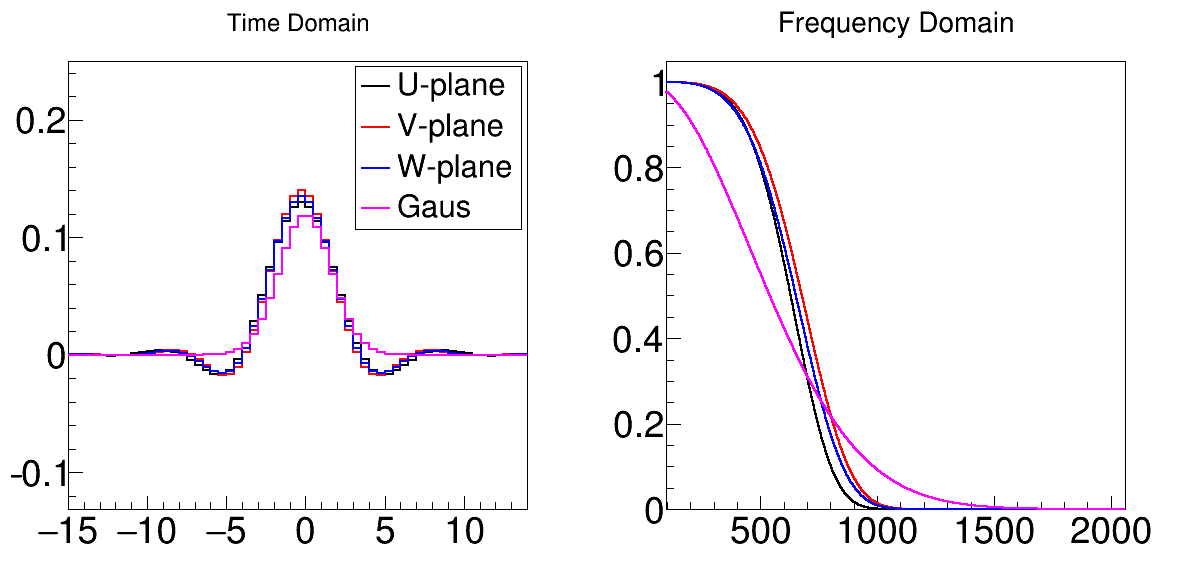
\includegraphics[width=0.8\textwidth]{filter_1.png}
\end{cdrfigure}

Beside the high-frequency software filter described above, there is also a low-frequency 
software filter which is used to select ROIs (discussed in Section~\ref{sec:decon-roi-selection}.) %the next section). 
The functional form of the low-frequency software filter is chosen to be 
\begin{equation}
F(\omega) = 1- e^{-\frac{1}{2}\cdot \left( \frac{\omega}{c} \right)^2}.
\end{equation}

%%%%%%%%%%%%%%%%%%%%%%%%
\subsection{ROI Selection}
\label{sec:decon-roi-selection}

The region of interest (ROI) is an important technique for limiting the contribution of low-frequency 
electronic noise. The ROI selection was based on the deconvoluted results. Essentially, we perform
two rounds of deconvolution:
\begin{itemize}
\item 2D deconvolution with the balanced Garfield-simulated field response function with a low-frequency filter (``2D deconvolution with low-frequency filter'').
\item 2D deconvolution with the balanced Garfield-simulated field response function without a low-frequency filter (``2D deconvolution'').
\end{itemize}
The first one is used to select ROIs, and the results from the second deconvolution are then 
used to obtain the final deconvoluted results. 

%%%%%%%%%%%%%%%%%%%%%%%%
\subsection{Metrics in Evaluating TPC Signal Processing}

In order to evaluate the TPC signal processing, which includes both the noise filtering and 
the charge extraction, two robust metrics can be used. % for evaluation purpose. 
They are:
\begin{itemize}
\item Equivalent Noise Charge (ENC): \\
  ENC is  basically proportional to the pedestal RMS in terms of ADC, and is a direct 
measure of the noise level in %the unit of 
electrons. It can be used to compare the 
noise levels from different experiments.
\item Deconvoluted Noise Charge after the TPC charge extraction (DNC): \\
The goal of the TPC charge extraction process is to recover the number of ionization 
electrons from the measured TPC signal. With the same procedure, the electronic noise
will also be converted. %The unit of these noise is again 
This is again measured in electrons, %which 
and so can be compared with 
the expected ionization electrons from energetic charged particles. 
The DNC depends on the ENC and on the frequency content of the noise spectrum. It also depends 
on the response function used for deconvolution, which is the primary reason 
why the induction plane DNC is much higher than the collection plane DNC. Furthermore, since
we have to rely on ROI and AB techniques to reduce the noise level for the induction plane, the
DNC also depends on the time-window length of the ROI. 
\end{itemize}
Understanding the ENC and DNC for the current-generation experiments and the expected 
performance for the future experiments are important steps to achieve automated event 
reconstruction for LArTPCs.

\begin{cdrfigure}[Residual noise vs wire length]{rms3}{The noise level in terms of the RMS value and ENC 
is plotted with respect to the wire length observed in MicroBooNE. 
This plot is taken from~\cite{noise_filter}.}
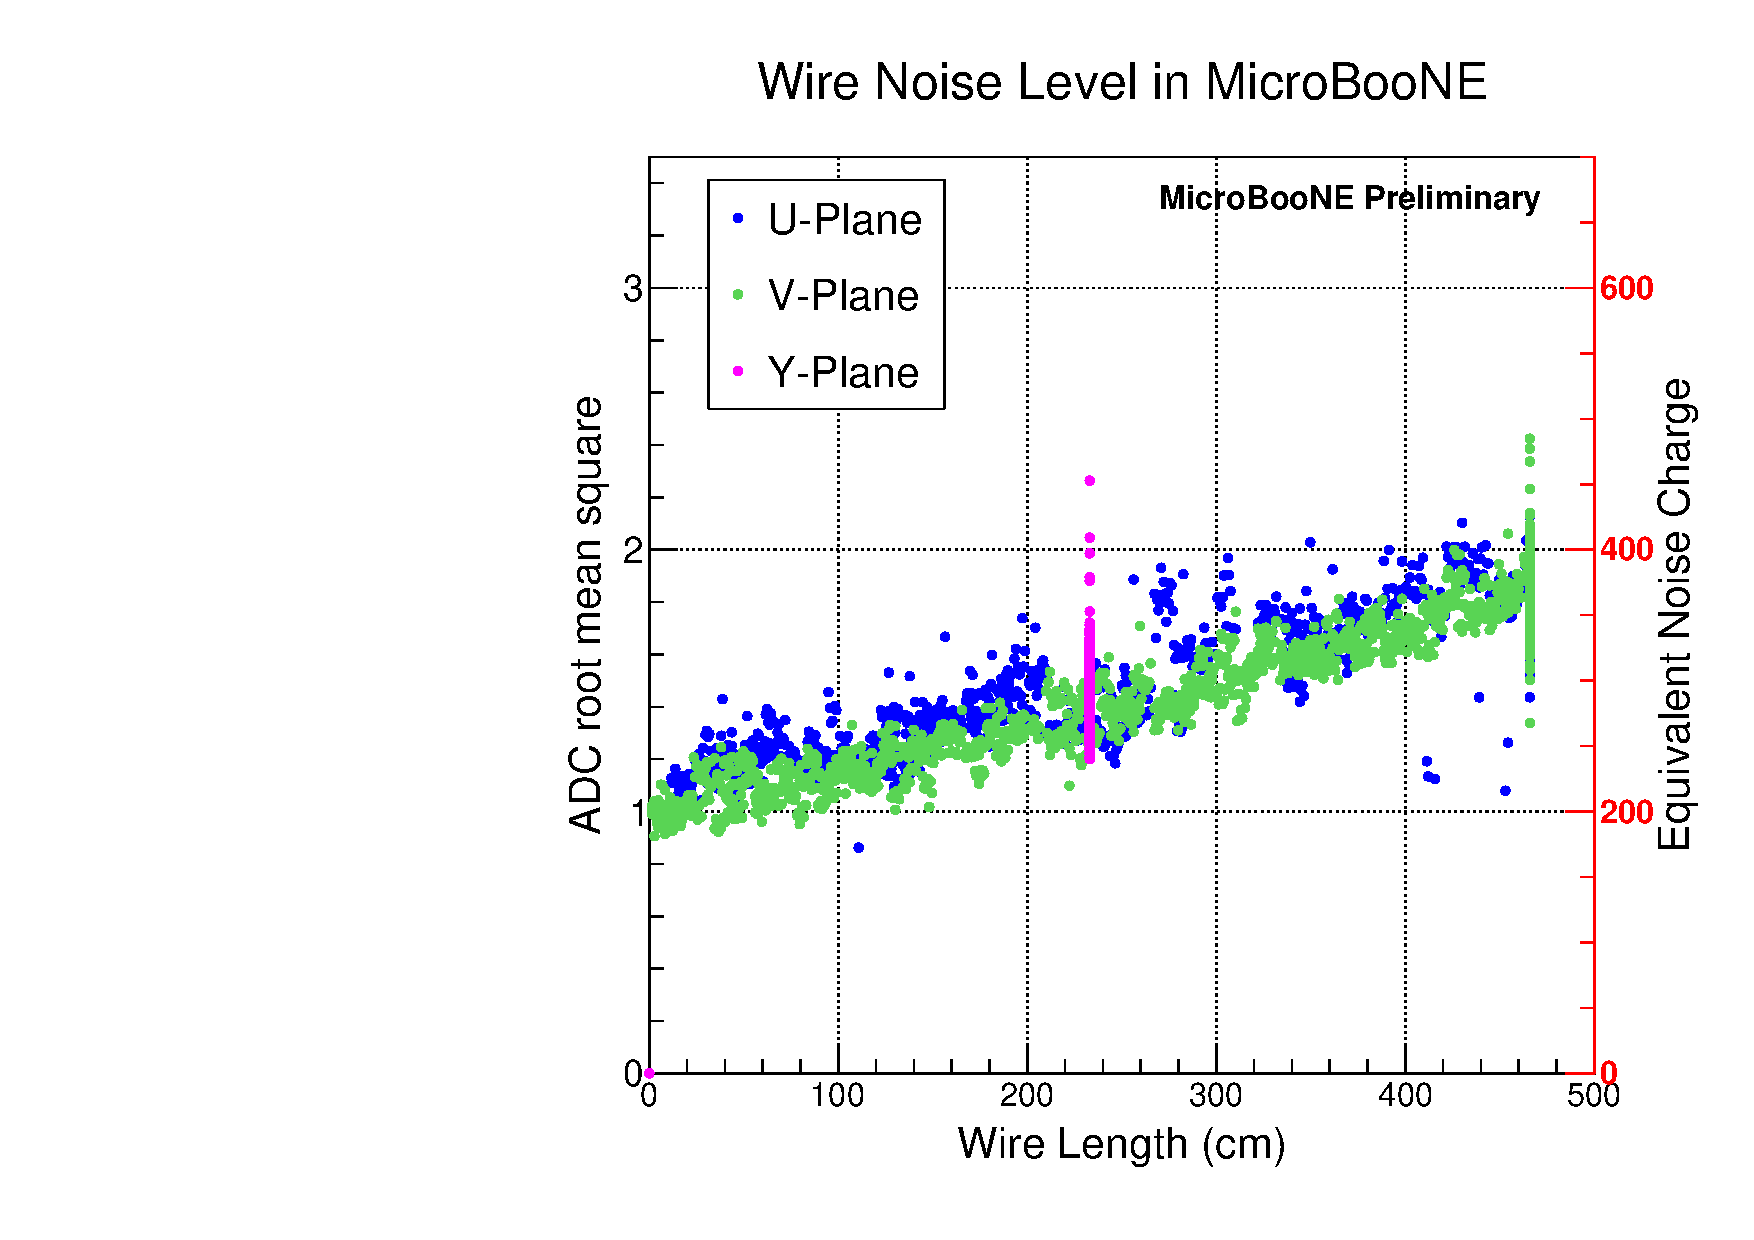
\includegraphics[width=0.75\textwidth]{RMSvsLength_after.pdf}
\end{cdrfigure}

The ENC in MicroBooNE has been reported at~\cite{noise_filter} and plotted 
in Figure~\ref{rms3}. As illustrate above \fixme{reference section or figure}, the calculation of the DNC depends on the 
drifted-charge extraction procedure. More specifically, it depends on the field 
response, the noise level (ENC and the frequency content), and the length of the ROI. 
Figure~\ref{DNC} shows the calculated DNC as a function of the time-window length 
for the second induction (V) plane, which is expected to have the smallest field 
response function (thus the largest DNC). 

\begin{cdrfigure}[Calculation of DNC vs time window length for second induction (V) plane]{DNC}{Calculation of DNC with respect to the time window length for second induction (V) plane. 
The ENC used in this simulation is 500 electrons given the induction wire length in protoDUNE. 
The red line shows the expected signal size for a minimal ionizing particle (MIP) 
traveling 3.2 mm.}
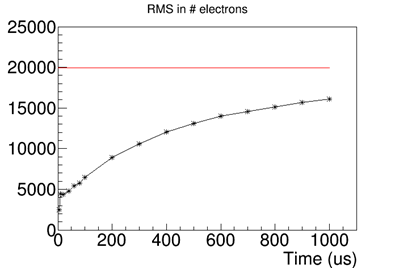
\includegraphics[width=0.75\textwidth]{DNC.png}
\end{cdrfigure}


